\chapter{Results and Analysis}

After the implementation phase of the design discussed in the previous chapter, the next phase involved performing tests to check if the implementation worked. To recapitulate the problem statement intended to be solved through the thesis was to increase the performance of the cuttlefish application by adding more computational capacity and distributing the objects to utilize the added computational power. The first part of the goal was achieved by creating a distributed system of heterogeneous systems as compute nodes connected through the enterprise network. For utilizing the computational capacity added, the application had to be modified to perform distribution of the work items amongst the computes nodes, collect their partial results and use the partial result to generate the final output. The desired result to be achieved through the thesis primarily was less computation time for multiple models as compared to computation time needed by current cuttlefish application and increase resource utilization by making use of the available machines.\newline

\section{Overview of SDLC Testing Phase} \label{SDLCTesting}

In the software development life-cycle, testing phase follows the implementation phase wherein various tests are conducted to verify and validate the implemented software. The result of the testing phase depends highly upon the type of test cases which are run. Testing can be classified into various categories depending on criteria chosen for classification, for example: the methods chosen to conduct tests, levels of testing etc. On the basis of methods used for testing, testing can be performed by manually testing the software or by automating the tests. In manual testing, the tester uses the software as an end-user and makes note of the deviations(if any) seen in the behavior of the system as from the expected. In automated testing, another software or scripts are used to run the various test-cases for the software under consideration. Each of these broadly classified types of testing techniques can consists of unit testing, integration testing, system testing, performance testing, regression testing etc.\newline

Manual testing as stated earlier is done by the tester by running the various use-cases in which an end user might execute the system. Mostly, manual testing is done to verify the system's behavior with respect to the specification which involves unit testing, integration testing. The validation of the implementation is done with respect to satisfying the needs of the customer which generally involves user acceptance tests and usability tests. Automated testing is generally done to perform regression testing where in part of the software under consideration is being fixed for some bug found by verification process, by re-writing a piece of code or introducing the fix by a new piece of code. The goal of regression tests is to ensure that the fixed bug is not leading to newer bugs in the system and thus is done quite frequently i.e. each time a discovered bug is fixed. Automation testing is also used to conduct stress test or performance tests where in the system is subjected to different loads and the behavior is observed with the primary goal to measure the performance or efficiency of the system under varying loads. As automation testing involves using other software or scripts to perform the tests, it cheaper and efficient both in terms of money and time. \newline 

On the basis of level of testing, testing can be done to check the functional or non-functional requirements. Functional requirements cover what the software is intended to do i.e. for a given input, the systems performs the intended task and the results generated by the system are correct. Non-functional requirements from the system involve checking the performance of the system, the resource utilization etc. \textbf{Functional testing} can broken down further into discrete levels as follows: 

\begin{itemize}
\item{\textbf{Unit Testing}}- Generally, it is performed by the developer who is aware about the code and the new modules which are implemented. The unit which is tested is generally doing a particular task / dedicated task and is a smaller portion of the whole code. The goal of the test is to ensure that each unit is performing the functionality it is implemented for. Unit tests generally have quite limited scope as it is not possible to cover all the execution paths of a code and the test data used by the developer is not the same as the test data to be used by the quality assurance team. 
\item{\textbf{Integration Testing}}- As the name suggests, integration testing is done to check if the individual modules tested via unit testing work correctly in unison. The unit testing of lower-level modules can be done first followed by integration tests by combining one or more modules which is called as bottom-up approach. If all the system modules together are tested i.e. the highest-level of module is tested first followed by testing each module individually later, it is called top-down approach.
\item{\textbf{System Testing}}- System testing is generally done by a specialized quality assurance team where in the system is tested as a whole to check if the system meets the quality standards agreed upon. The system is tested in an environment which is very similar to the production environment i.e. the environment where the developed application is going to be deployed.
\item{\textbf{Acceptance Testing}}- One of the most crucial steps of testing, the QA team verifies if the application works correctly for test scenarios which are discussed prior to the implementation by the customer and the development team. These test cases are drawn on the basis of the acceptance criteria for the software. 
\end{itemize}        

\textbf{Non-Functional testing} as mentioned earlier includes testing the non-functional requirements of the software such as the performance of the system, security, ease of use of the system etc. Non-Functional testing can be broken down into following levels: 

\begin{itemize}
\item{\textbf{Performance Testing}}- Performance testing involves exposing the system under consideration to various levels of stress and loads to monitor the behavior of the system. The goal of this type of testing is to identify the performance issues or bottlenecks which could be caused by network delay, large data input size, hitting peak processing capacity etc.  
\item{\textbf{Usability Testing}}- This type of testing involves the checking the ease of use for the software where the possible improvements in the software are noted by observing the users use the software. It involves checking the efficiency of use, learn-ability, error messages seen by the user and satisfaction of the user.
\item{\textbf{Portability Testing}}- If the software is built with multi-platform support, then this type of testing checks the functioning of the software on different platforms. The diversity in the platforms covers checking different operating systems, different underlying architecture or type of network.    
\item{\textbf{Security Testing}}- The intention of security testing is to find any vulnerabilities in the software which would compromise the security guarantees that should be provided by the software. The checks are done to ensure confidentiality, integrity, authentication, availability, authorization, non-repudiation, buffer over-flow vulnerabilities etc. 
\end{itemize} 

\section{Implementation Assessment}

Amongst the types of testing discussed in the Section \ref{SDLCTesting}, the implementation of the thesis was tested by using manual testing during the development and automated testing after the development was done. The manual testing involved running the scenarios to check individual components or parts of the components.  
Following the unit tests, were the tests which involved checking how the components worked together for different scenarios. Some of the manual tests performed are described in Section \ref{ManualTests}. The performance of the distributed cuttlefish is measured through automated testing. The performance tests and results of the tests are discussed in the Section \ref{PerformanceTests}.

\subsection{Manual Tests} \label{ManualTests}

Out of the various test cases which were conducted, the important cases have been documented in this Section which highlight the scenarios testing the components newly introduced for distributed computing. 

\begin{enumerate}
\item{Test-cases specific for Prototype I}: The prototype I tests included testing the \textit{MasterDistributor}, \textit{SlaveReporter} and \textit{MasterMerger} components. 
\begin{itemize}
\item{\textbf{Test-Case for \textit{MasterDistributor} Component}}:

\begin{itemize}
\item{\textbf{Scenario}}- To test if the \textit{MasterDistributor} component generates correct distribution for a given set of input objects and cluster size. The goal is to test the correct calculation of the threshold function, creation of distributed print object list and using the generated list correctly writing the main configuration file for each slave node.  
\item{\textbf{Method}}- Distributed cuttlefish was executed multiple times with varying inputs. The test data for the simplest scenario consisted of 2 head models to be distributed among 3 node cluster with 2 slaves and one master node. Each head was 8cms and the expected balanced distribution of the input would to be generate load of one head model per slave node. The same test case was run repeatedly with varying the number of input objects, different types of input models i.e. varying the test-data and cluster size. 
\item{\textbf{Results}}- As in prototype I, the \textit{MasterDistributor} component generated main configuration file per slave and the output of the current test was verified by checking the number of print objects in the main configuration file for each slave node. Another way to check the threshold calculation was to use simple standard output statements or logging the information in a trace file.
\end{itemize}

\item{\textbf{Test-Case for \textit{SlaveReporter} Component}}: 
\begin{itemize}
\item{\textbf{Scenario}}- The \textit{SlaveReporter} Component generates the output with partial slices, which are written to the disk after serialization and chunk-wise sending the path to the master. To test if the \textit{SlaveReporter} component generates correct partial output and the path sent to the master is the correct location.
\item{\textbf{Method}}- Distributed cuttlefish was executed on the slave node. To check if the serialization of the partial slices happens correctly, the slices are deserialized at the slave and the partial output is written to the disk as images. The part of code implementing the test i.e. deserialization of the slices and generating images of the partial slices is not part of the final code which is used to build the distributed cuttlefish binary but is rather just code to test the scenario. 
\item{\textbf{Results}}- The images of the partial slices generated by the \textit{SlaveReporter} component were thoroughly checked to ensure correct material assignment. Ensuring that the partial slices are correctly serialized helped to narrow down the errors which were encountered in generation of the merged slices.  
\end{itemize}

\item{\textbf{Test-Case for \textit{MasterMerger} Component}}: 
\begin{itemize}
\item{\textbf{Scenario}}- The \textit{MasterMerger} Component generates the output with merged slices, which are written to the disk in a chunk-wise fashion after de-serialization. To test if the \textit{MasterMerger} component generates correct merged output.
\item{\textbf{Method}}- Distributed cuttlefish was executed in the cluster.To check if the de-serialization of the partial slices happens correctly at the master, the de-serialized partial slices are written to the disk as images before writing to the merged full slices. The part of code implementing the test i.e. deserialization of the slices and generating images of the partial slices is not part of the final code which is used to build the distributed cuttlefish binary but is rather just code to test the scenario. 
\item{\textbf{Results}}- The images of the partial slices generated by the \textit{MasterMerger} component were thoroughly checked to ensure correct material assignment. The final output of the \textit{MasterMerger} component i.e. the merged full slices were verified by checking the output of the \textit{SliceDebug} component output. Through this test a bug in the code was detected wherein the empty full slices created before writing the partial slices were not initialized with empty voxel value i.e. no material assigned these voxels, leading to random value assignment to them which lead to incorrect results, i.e. slices had random patches of materials assigned. 
\end{itemize}
\end{itemize}  

\item{\textbf{Test-cases specific for Prototype II}}: The testing of prototype II was done through the test cases for \textit{MasterPJDistributor}, \textit{SlavePJCollector}, \textit{SlaveReporter} and \textit{MasterMerger} 

\begin{itemize}
\item{\textbf{Test-Case for \textit{MasterPJDistributor} Component}}:

\begin{itemize}
\item{\textbf{Scenario}}- To test if the \textit{MasterPJDistributor} component generates correct distribution for a given set of input objects and cluster size. The goal is to test the correct calculation of the threshold function, creation of distributed print object list and using the generated list correctly to generate the print job per slave node.
\item{\textbf{Method}}- Distributed cuttlefish was executed multiple times with varying inputs. The test data for the simplest scenario consisted of 2 head models to be distributed among 3 node cluster with 2 slaves and one master node. Each head was 8cms and the expected balanced distribution of the input would to be generate load of one head model per slave node. The same test case was run repeatedly with varying the number of input objects, different types of input models i.e. varying the test-data and cluster size. 
\item{\textbf{Results}}- As in prototype II, the \textit{MasterPJDistributor} component generated print job per slave and the output of the current test was verified by debugging the number of print objects in the print job for each slave node. Another way to check the threshold calculation was to use simple standard output statements or logging the information in a trace file. Through this test, a bug in the code which led to incorrect threshold calculation was caught. The incorrect threshold calculation lead incorrect number of print objects in the print jobs leading to one of the computes nodes being overloaded. Another bug related to placement of the print objects in the print bed was discovered as well, where in the print jobs sent to the slaves had print objects with the transformation created by the print job organizer at the master. This lead to generation of partial slices with the print objects placed at some displacement from the origin at the slave. This bug was later fix by changing the behavior of the \textit{MasterMerger} component for prototype II.
\end{itemize}

\item{\textbf{Test-Case for \textit{SlavePJCollector} Component}}:

\begin{itemize}
\item{\textbf{Scenario}}- To test if the \textit{SlavePJCollector} component receives correct input from the master. The goal is to test if the \textit{SlavePJCollector} component correctly receives the serialized print job, deserializes the print job and loads the texture information to the GPU memory after receiving it from the master and deserializing the received texture data.
\item{\textbf{Method}}- Distributed cuttlefish was executed multiple times on the slave node with varying number of input models at the master.
\item{\textbf{Results}}- In the prototype II, the \textit{SlavePJCollector} component receives the serialized print job from the master. The size of the serialized data was cross-examined with the size of data sent at the master node. After deserializing the print job, the number of print objects contained in the print job was checked through debugging the component. To check if the texture data was received and deserialized correctly, the deserialized data was written to an image on the disk. Through this test, a bug in the format in which the texture data was uploaded to the GPU memory at the slave node was found. The texture data is in RGBA format and is linearized at the master node before uploading the data to master node GPU. When the texture data is communicated to the slave, the load operation should not perform the linearization again and instead load the data directly to the GPU memory.
\end{itemize}
\end{itemize} 

\item{\textbf{Test-Cases Common for Prototype I and Prototype II}}:
There are some corner cases which had to be checked for both the prototypes. These scenarios and the tests performed to check how the system handles these scenarios are described as follows:

\begin{itemize}
\item{\textbf{Corner Case I}- Size of input objects < number of slave nodes }
\begin{itemize}
\item{\textbf{Scenario}}- To test the behavior of distributed cuttlefish when the number of input objects submitted to the master node is smaller than the cluster size i.e. number of print objects in the main configuration file are less than the number of slave nodes.
\item{\textbf{Method}}- Distributed cuttlefish was executed with submitted main configuration file consisting of less number print objects in comparison to the number of nodes given to mpiexec command, i.e.  cluster size is number of print objects plus 2 (as master node does not act as a slave node)
\item{\textbf{Results}}- When the number of print objects is less than the number of available slave nodes, some of the slave nodes get empty input. At the master, the \textit{MasterMerger} component is notified the number of slaves nodes doing the actual work so as to ensure that the \textit{MasterMerger} component waits to receive the partial slices only from these many slave nodes. For prototype I, the empty work item to the {\lq}dropped{\rq} slaves is given by writing a main configuration file without any print object files. Through this test case, it was discovered that the cuttlefish application did not handle empty input case and crashed. So to handle the empty input, there were some modifications introduced in the application. For Prototype II, the empty input the {\lq}dropped{\rq} slaves is given by sending a print job without any print objects. The {\lq}dropped{\rq} slaves do execute the whole pipeline once with null input and wait for the other slaves doing the work to finish while they execute MPI\_Barrier call.     
\end{itemize}
\item{\textbf{Corner Case II}- Size of input objects = 1}
\begin{itemize}
\item{\textbf{Scenario}}- To test the behavior of distributed cuttlefish when only one print object is submitted to the master node, i.e.the main configuration file contains only one print object file.
\item{\textbf{Method}}- Distributed cuttlefish was executed with submitted main configuration file consisting of 1 print object.
\item{\textbf{Results}}- Irrespective of the number of slave nodes in the cluster, as there is only one print object provided as input to the distributed cuttlefish, there is no need to calculate the threshold to perform the distribution. So, the slave node with rank 1 i.e. the first slave node in the cluster gets the print object and rest of the slave nodes (if any depending on the number of hosts set in the mpiexec command) are {\lq}dropped{\rq} and the behavior of the system is similar to the behavior discussed in the above test-case.
\end{itemize}

\item{\textbf{Corner Case III}- No input given to the distributed cuttlefish}
\begin{itemize}
\item{\textbf{Scenario}}- To test the behavior of distributed cuttlefish when input of size is 0.
\item{\textbf{Method}}- Distributed cuttlefish was executed with submitted main configuration file consisting of 0 print objects.
\item{\textbf{Results}}- When the input size is 0, for prototype II, the \textit{MasterPJDistributor} component gets an empty print job from the \textit{PrintJobOrganizer} component. The \textit{MasterPJDistributor} component informs the \textit{MasterMerger} component that all the slave nodes are dropped and it should not wait for any partial output from the slave nodes. For prototype I, all the slave nodes receive empty configuration files and the master behaves the same as in prototype II. 
\end{itemize}
\end{itemize}
\end{enumerate}

 
\section{Results} \label{PerformanceTests}

The performance testing is done through automation of the test-cases. To perform automated testing, either another software is used to run the software under test or scripts are written to perform the testing. For testing the distributed cuttlefish, batch scripts were written and executed to perform the tests. For each test case, the test-data was created along with the script and the task was scheduled using the windows task scheduler. The performance tests were conducted to check the computation speed-up and efficiency achieved by distributed computing. The Section \ref{DistvsNonDist} explains the terms computational speed-up and efficiency in parallel computing followed by the test case used to find the speed-up and observed result. The Section \ref{ProtoComp} details the comparison of the two prototypes developed in terms of computation speed-up, communication overhead and how well the prototypes scale for a given work load.

\subsection{Comparison of distributed vs non-distributed cuttlefish performance} \label{DistvsNonDist}

Speed-up is one of the most common metric used to measure performance of a parallel processing and is defined as the gain by parallel computation in terms of performance in comparison to the sequential computation. \textit{Absolute speed-up} calculation can be done by considering how fast the computation can be performed by using N processors in comparison to best sequential algorithm performance on a single processor \cite{Speedup}. \textit{Relative speed-up }is defined as the ratio of performance of parallel algorithm on one processor to the performance of same on N processors. \textit{Relative speed-up} is used to compare how well the algorithm performs when the number of processors is scaled up \cite{Speedup}. To do performance evaluation for distributed cuttlefish, we use the absolute speed-up definition and Equation \ref{eq:speed-up} to calculate the speed-up, where N is number of processors, \begin{math} T_{s} \end{math} - is the execution time of non-distributed cuttlefish for the given work load, \begin{math} T_{N}\end{math}- is the execution time of distributed cuttlefish for the same work load.

\begin{equation}
\label{eq:speed-up}
\begin{aligned}
S_{N} = T_{s}/T_{N}
\end{aligned}
\end{equation}

Using the Equation \ref{eq:speed-up}, the speed-up can be classified as either linear speed-up, sub-linear speed-up or super-linear speed-up. Linear speed-up is observed when \begin{math}S_{N}=N \end{math} i.e. speed-up is equal to the number of processors. Sub-linear speed-up is when the speed-up is lesser than number of processors where are super-linear speed up is when the speed-up gained is larger than the number of processors. Some of the reasons why super-linear speed-up is possible are higher cache hit rate, better resource utilization, lower network latency for small-sized messages communication. The Figure summarizes the three types of speed-up observed. \newline 

\begin{figure}[t]
\centering
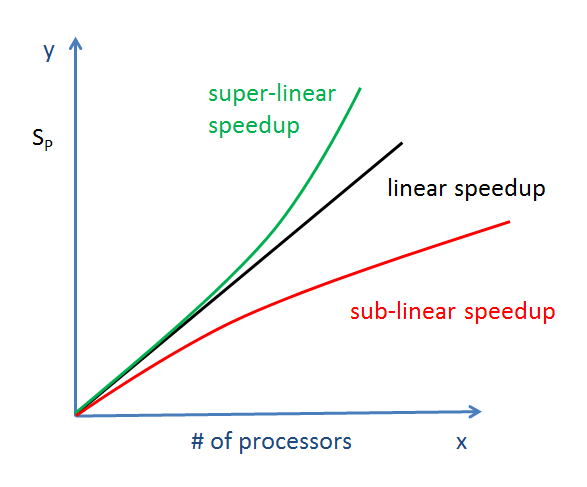
\includegraphics[scale=0.8]{TypesOfSpeedUp.PNG}
\caption{Speed-Up Types}
\label{fig:TypesOfSpeedUp}
\end{figure}

Efficiency is defined as a ratio of speed-up gained for \textit{N} processors to the number of processors. The Equation \ref{eq:eff} is used to calculate the efficiency.

\begin{equation}
\label{eq:eff}
\begin{aligned}
E_{N} = S_{N}/N
\end{aligned}
\end{equation}

\subsubsection{Distributed Cuttlefish Prototype I vs Non-Distributed Cuttlefish}

To check the speed-up gained by using the Distributed Cuttlefish Prototype I, the application was run with different work-loads and comparison between the execution times for both Distributed Cuttlefish Prototype I and Non-Distributed Cuttlefish application was drawn.

\begin{enumerate}
\item{\textbf{Scenario}}- To test the computational speed-up gained by distributed cuttlefish prototype I in comparison to non-distributed cuttlefish for input consisting of same models.
\begin{itemize}
\item{\textbf{Test-Case and Test-Data Description}}- The test case was executed 5 times for each test-data. The cluster was composed of 3 nodes where in one node was the master and remaining two were compute nodes. The cluster nodes were heterogeneous in terms of the number of cores, CPU speed and RAM capacity. The test-data included multiple head models of size 8cms. The number of head models was increased by factor of 2 for each following test-case, i.e. starting with 2 head models the number was increased to 10 head models for the 5 test-cases, with each test-case executed 5 times to enable collection of the average execution times. The speed-up for each test case was calculated using the average execution time for distributed cuttlefish and non-distributed cuttlefish for a given test-data i.e. given work-load. The non-distributed cuttlefish application was executed on the slowest node of the cluster as the slowest node in the cluster would impact the execution time of the distributed version. 
\item{\textbf{Results}}- To elaborate on the amount of work to be done, each 8 cm head model consists of 777 slices with each slice having the width-946 units (8.00 cm)and height-303 units (5.12 cm). The total number of voxels for each model is calculated using the Equation \ref{eq:NumVoxel} where, \begin{math} T_{NumVoxels} \end{math} is the total number of voxels for a given model, width (W), height(H), length (L) and voxel dimensions (voxDims). For each head model used in the test data, the total number of voxels to be processed is \begin{math} 2.17 \times 10^{8} \end{math}. Each voxel can be assigned values denoting the materials and a null material value depending upon the printer specification provided. For current test case, the materials provided in the printer specification are VeroCyan, VeroWhite, VeroMagenta, VeroYellow, VeroBlack and EMPTY\_VOXEL as null material . For each material there is a bitmap generated denoting the voxels which are assigned that particular material in the slice. Figure \ref{fig:SliceOutput} shows the material assignment generated for 108th slice of a single head model. The Table \ref{protoIvsND} summarizes the execution times for distributed cuttlefish with prototype I and non-distributed cuttlefish along with the speed-up.  
\item{\textbf{Observation}}- The number of slave nodes is constant throughout the test-cases i.e. 2 slave nodes and the work-load provided to the system is increased for every test-case. The speed-up is calculated as per the Equation \ref{eq:speed-up} and increases with the increase in work-load in comparison to the non-distributed cuttlefish performance. The Figure \ref{fig:ProtoISpeedupVsNumModels} depicts the scaling of the speed-up with increase in work load i.e number of models. The Figure \ref{fig:ProtoISpeedupVsNumModels}shows some interesting results, the speed-up seen is linear with increase in work-load until it reaches a point where in for a given cluster size increase in the load does not provide linear increase in speed-up although the distributed cuttlefish prototype I performs better than non-distributed version. This is proved by calculating the efficiency using the Equation \ref{eq:eff} and by seeing the trend depicted in the Figure \ref{fig:EfficiencyVsNumModels}. 
\end{itemize}

\item{\textbf{Scenario}}- To test the computational speed-up gained by distributed cuttlefish prototype I in comparison to non-distributed cuttlefish for input consisting of different models.
\begin{itemize}
\item{\textbf{Test-Case and Test-Data Description}}- The test case was executed 5 times for each test-data. The cluster was composed of 3 nodes where in one node was the master and remaining two were compute nodes. The cluster nodes were heterogeneous in terms of the number of cores, CPU speed and RAM capacity. The test-data included multiple head and dame models of size 8 cm. The number of models was increased by factor of 2 for each following test-case, i.e. starting with 1 head model and 1 dame model, the number was increased to 5 head and dame models each, for the 5 test-cases, with each test-case executed 5 times to enable collection of the average execution times. The speed-up for each test case was calculated using the average execution time for distributed cuttlefish and non-distributed cuttlefish for a given test-data i.e. given work-load. The non-distributed cuttlefish application was executed on the slowest node of the cluster as the slowest node in the cluster would impact the execution time of the distributed version. 
\item{\textbf{Results}}- To elaborate on the amount of work to be done, each 8cms head model consists of 777 slices, with each slice having the width-946 units (8.00 cm)and height-303 units (5.12 cm). The total number of voxels for each model is calculated using the following Equation \ref{eq:NumVoxel} where, \begin{math} T_{NumVoxels} \end{math} is the total number of voxels for a given model, width (W), height(H), length (L) and voxel dimensions (voxDims). For each head model used in the test data, the total number of voxels to be processed is \begin{math} 2.17 \times 10^{8} \end{math}. Each 8 cm dame model consists of 605 slices, with each slice having the width-946 units (8.00 cm)and height-194 units (3.27035 cm). The total number of voxels for the dame model calculated using the Equation \ref{eq:NumVoxel} is  \begin{math} 1.09495848 \times 10^{8} \end{math}. Each voxel can be assigned values denoting the materials and a null material value depending upon the printer specification provided. For current test case, the materials provided in the printer specification are VeroCyan, VeroWhite, VeroMagenta, VeroYellow, VeroBlack and EMPTY\_VOXEL as null material . For each material there is a bitmap generated denoting the voxels which are assigned that particular material in the slice. The Table \ref{protoIvsNDDiffModel} summarizes the execution times for distributed cuttlefish with prototype I and non-distributed cuttlefish along with the speed-up for input consisting of different models.  
\item{\textbf{Observation}}-  The number of slave nodes is constant throughout the test-cases i.e. 2 slave nodes and the work-load provided to the system is increased for every test-case. The speed-up is calculated as per the Equation \ref{eq:speed-up} and increases with the increase in work-load in comparison to the non-distributed cuttlefish performance. Although, the speed-up achieved for a given number of models with input consisting of only head models was marginally more than the speed-up achieved when distributed cuttlefish was executed with equal number of models with input consisting of different models. The Figure \ref{fig:SpeedUp-ProtoIDiffModelsVsNumModels} depicts the scaling of the speed-up with increase in work load i.e number of models. Unlike the plot seen in Figure \ref{fig:ProtoISpeedupVsNumModels}, the speed-up increases with increase in the work-load and there is no drop in the speed-up.This is proved by calculating the efficiency using the Equation \ref{eq:eff} and by seeing the trend depicted in the Figure \ref{ProtoIDiffModelsVsNumModels}. 
\end{itemize}
\end{enumerate}

\begin{table}[]
\centering
\caption{Speed-Up \& Efficiency: Distributed Cuttlefish Prototype I vs Non-Distributed Cuttlefish For Same Models}
\label{protoIvsND}
\begin{tabular}{|c|l|l|l|c|}
\hline
\textbf{\begin{tabular}[c]{@{}c@{}}Number of \\ Head Models\\ 8cms\\ (Resolution:\\ 300 X 150 X 470)\end{tabular}} & \multicolumn{1}{c|}{\textbf{\begin{tabular}[c]{@{}c@{}}Total Execution Time (in Secs)\\  for Distributed \\ Cuttlefish Prototype I\\ (Cluster Size- 3)\end{tabular}}} & \multicolumn{1}{c|}{\textbf{\begin{tabular}[c]{@{}c@{}}Total Execution Time (in Secs) \\ for Non-Distributed\\ Cuttlefish\end{tabular}}} & \multicolumn{1}{c|}{\textbf{Speed-Up}} & \textbf{Efficiency} \\ \hline
2                                                                                                                  & 173.3568                                                                                                                                                    & 357.3552                                                                                                                       & 2.0614652                              & 0.6871551           \\ \hline
4                                                                                                                  & 363.3992                                                                                                                                                    & 920.566                                                                                                                        & 2.5332101                              & 0.8444034           \\ \hline
6                                                                                                                  & 585.3218                                                                                                                                                    & 1651.1775                                                                                                                      & 2.8209769                              & 0.9403256           \\ \hline
8                                                                                                                  & 836.2334                                                                                                                                                    & 4071.576                                                                                                                       & 4.8672945                              & 1.6224315           \\ \hline
10                                                                                                                 & 1130.514                                                                                                                                                    & 4790.198                                                                                                                       & 4.2371859                              & 1.4123953           \\ \hline
\end{tabular}
\end{table}


\begin{table}[]
\centering
\caption{Speed-Up \& Efficiency: Distributed Cuttlefish Prototype I vs Non-Distributed Cuttlefish For Different Models}
\label{protoIvsNDDiffModel}
\begin{tabular}{|c|l|l|l|c|}
\hline
\textbf{\begin{tabular}[c]{@{}c@{}}Number of \\ Head \& Dame\\  Models -8 cm\\ (Resolution:\\ 300 X 150 X 470)\end{tabular}} & \multicolumn{1}{c|}{\textbf{\begin{tabular}[c]{@{}c@{}}Total Execution Time \\ (in secs)\\  for Distributed \\ Cuttlefish Prototype I\\ (Cluster Size- 3)\end{tabular}}} & \multicolumn{1}{c|}{\textbf{\begin{tabular}[c]{@{}c@{}}Total Execution Time\\ (in secs) \\ for Non-Distributed\\ Cuttlefish\end{tabular}}} & \multicolumn{1}{c|}{\textbf{Speed-Up}} & \textbf{Efficiency} \\ \hline
2                                                                                                                            & 184.25                                                                                                                                                                   & 243.94                                                                                                                                     & 1.323962008                            & 0.441320669         \\ \hline
4                                                                                                                            & 315.342                                                                                                                                                                  & 635.524                                                                                                                                    & 2.015348415                            & 0.671782805         \\ \hline
6                                                                                                                            & 563.3                                                                                                                                                                    & 1171.32                                                                                                                                    & 2.079389313                            & 0.693129771         \\ \hline
8                                                                                                                            & 685.21                                                                                                                                                                   & 1890.706                                                                                                                                   & 2.759308825                            & 0.919769608         \\ \hline
10                                                                                                                           & 988.708                                                                                                                                                                  & 4793.47                                                                                                                                    & 4.848216056                            & 1.616072019         \\ \hline
\end{tabular}
\end{table}

\begin{figure}[t]
\centering
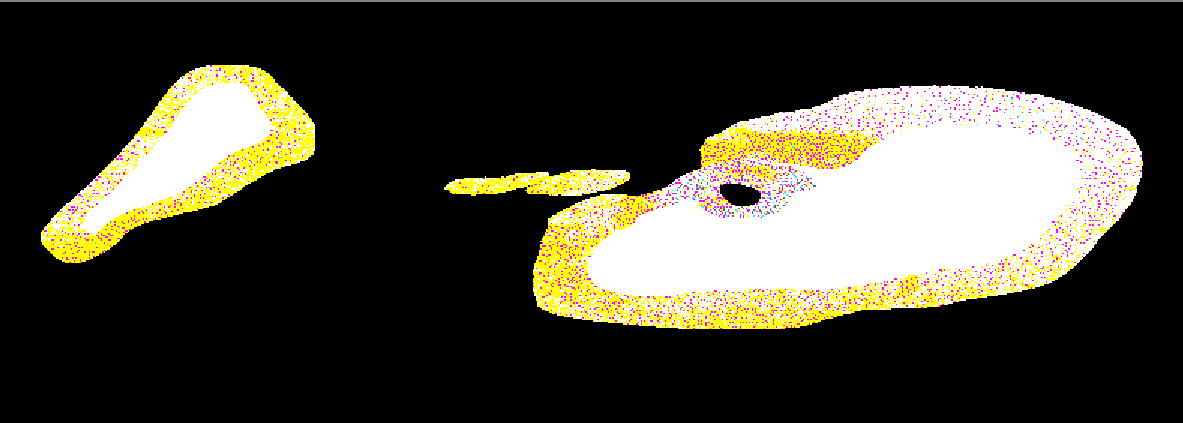
\includegraphics[scale=0.5]{SliceOutput.PNG}
\caption{Material Assignment for Single Slice}
\label{fig:SliceOutput}
\end{figure}

\begin{figure}
\centering

\begin{subfigure}
\centering
\captionsetup[subfigure]{labelformat=empty}
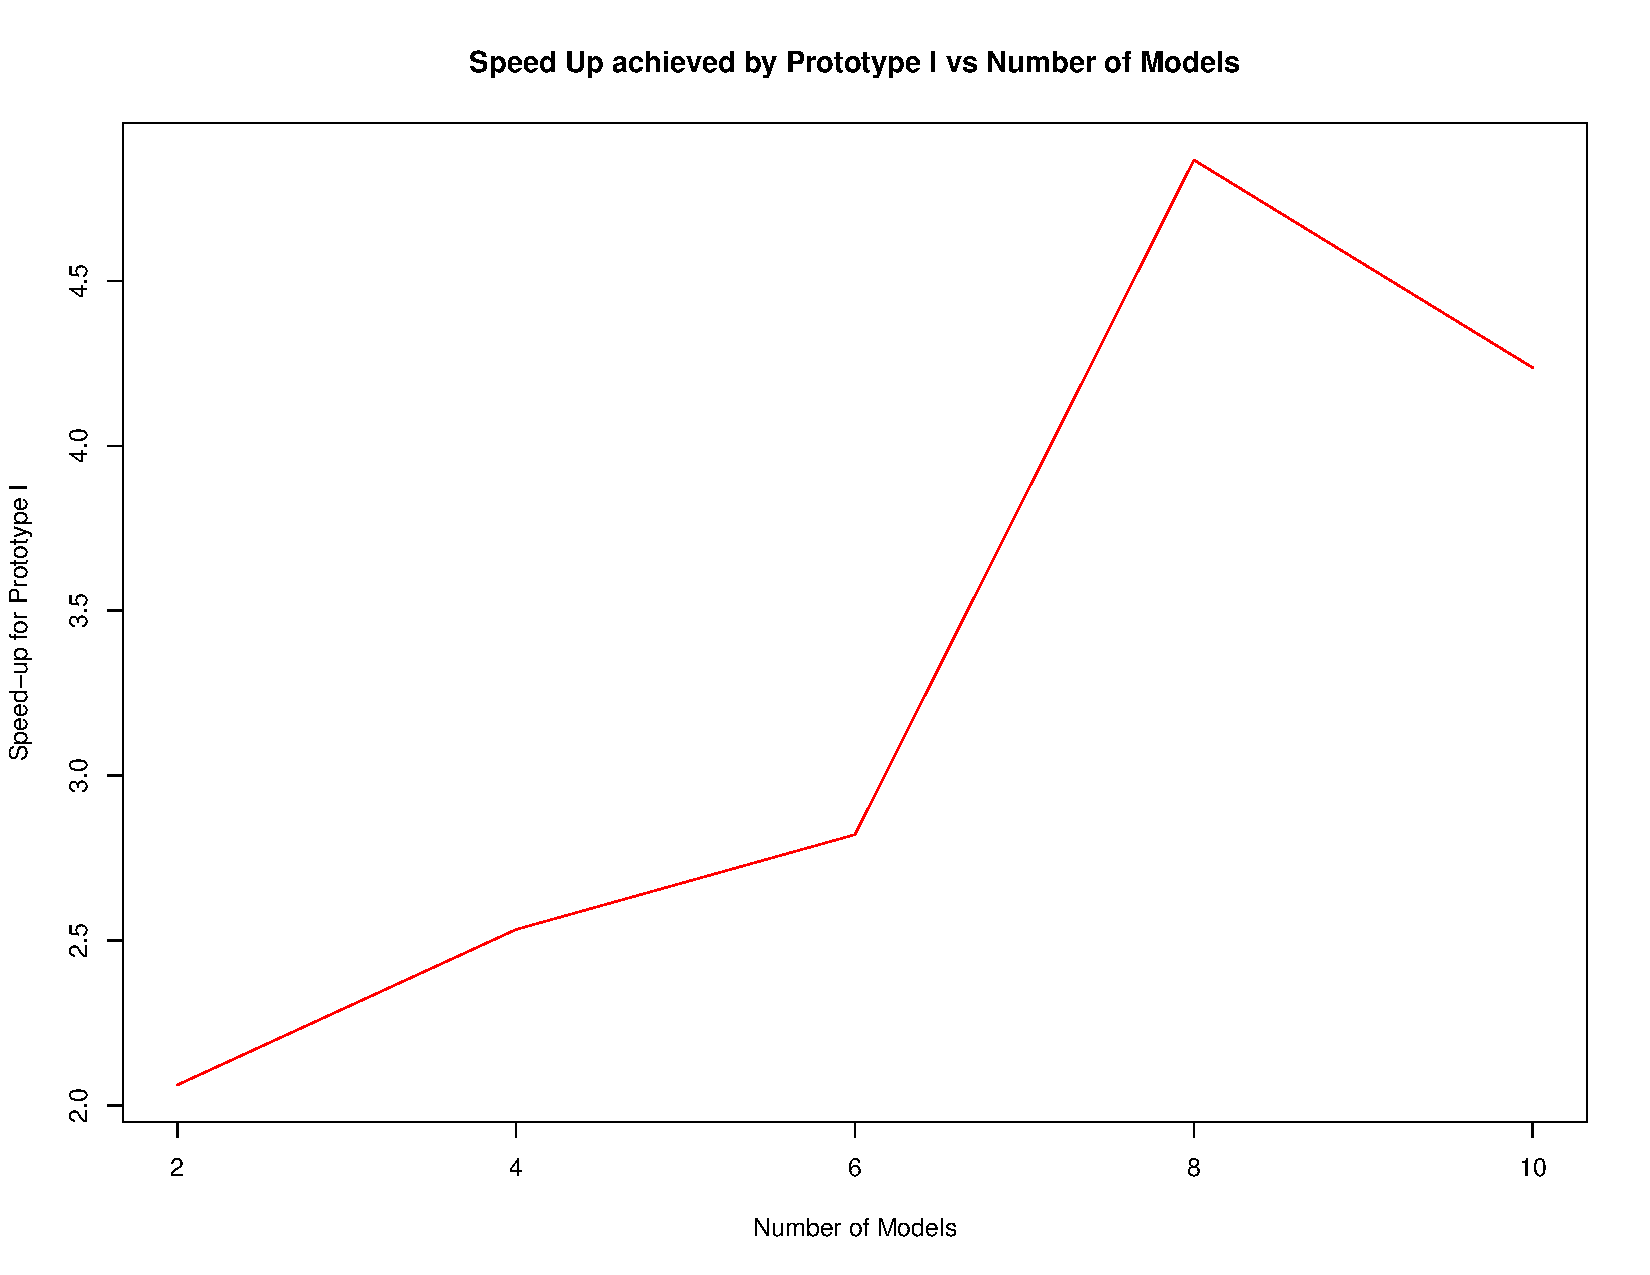
\includegraphics[scale=0.5]{ProtoISpeedupVsNumModels.pdf}
\caption{Speed-up Vs Number of Models}
\label{fig:ProtoISpeedupVsNumModels}
\end{subfigure}
\begin{subfigure}
\centering
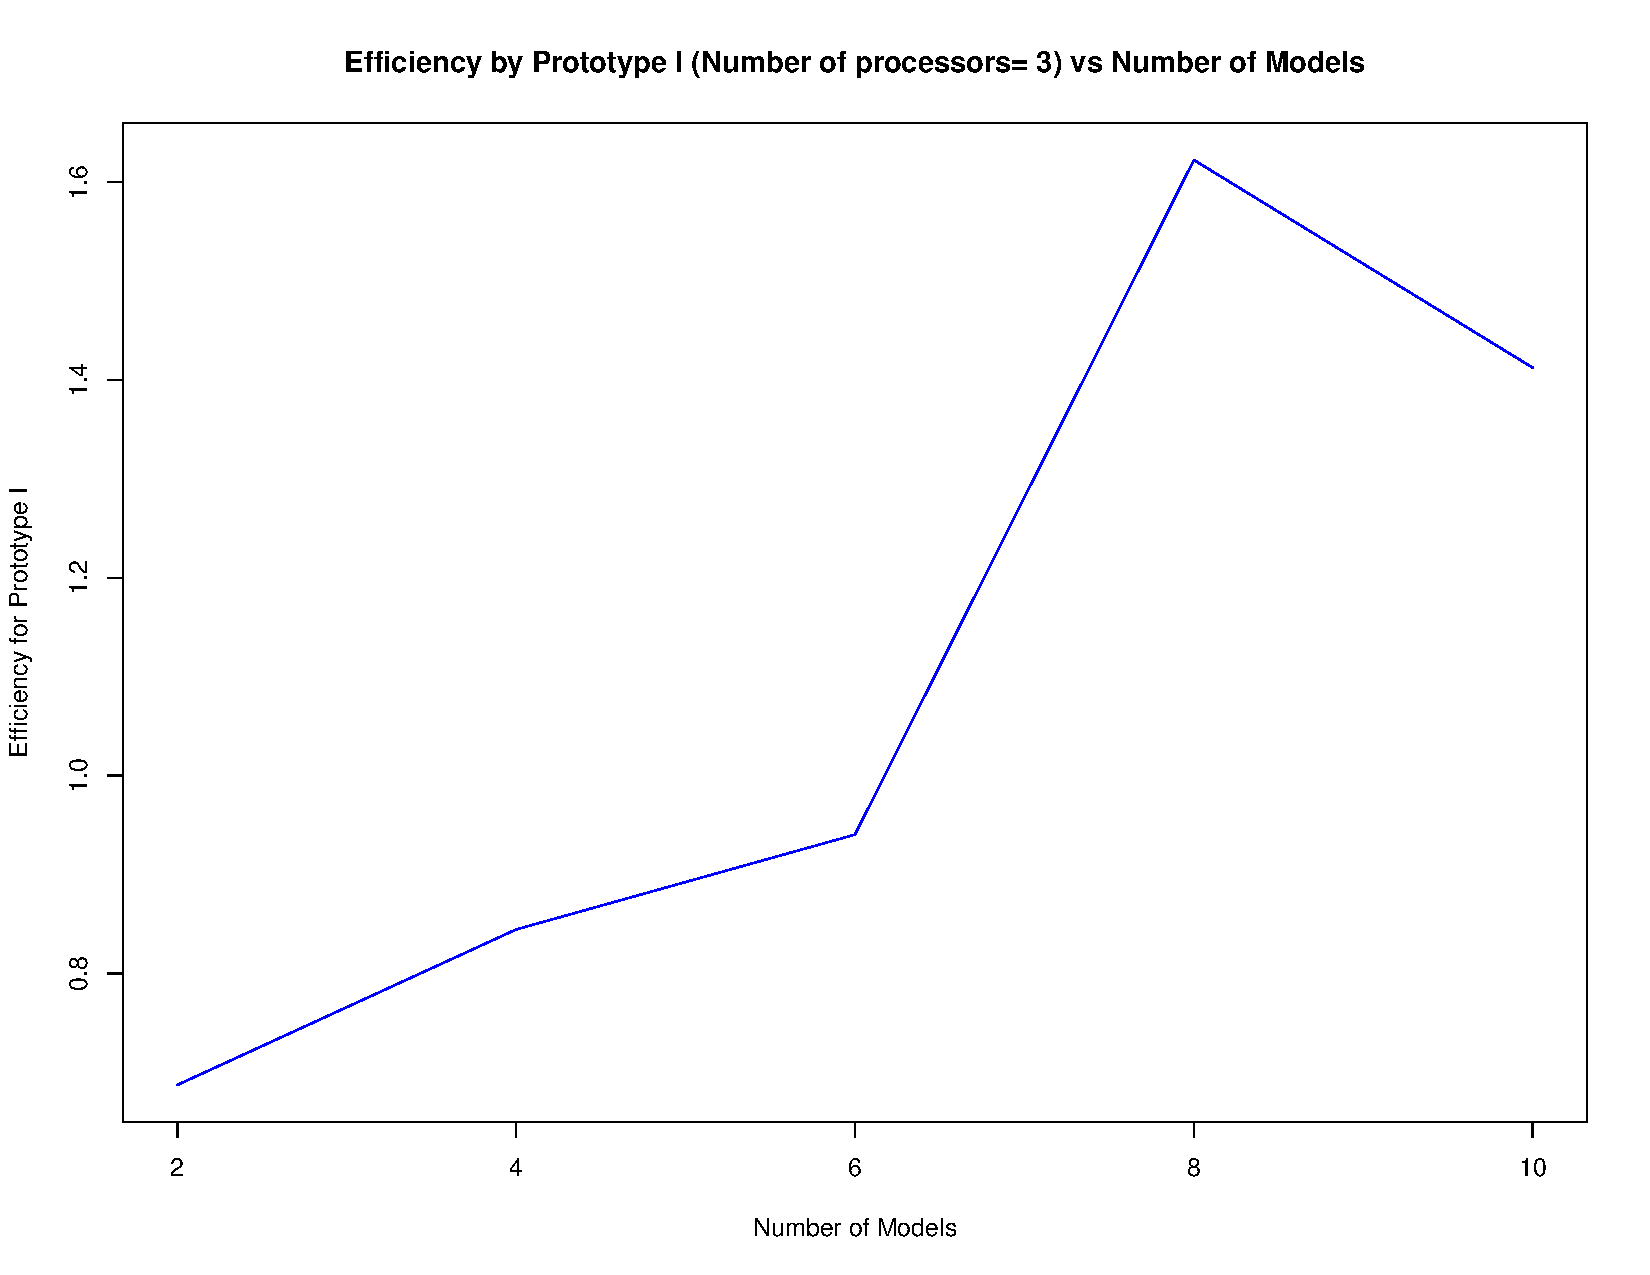
\includegraphics[scale=0.5]{EfficiencyPrototIvsNumModels.pdf}
\caption{Efficiency Vs Number of Models}
\label{fig:EfficiencyVsNumModels}
\end{subfigure}
\end{figure}


\begin{figure}
\centering
\captionsetup[subfigure]{labelformat=empty}
\begin{subfigure}
\centering
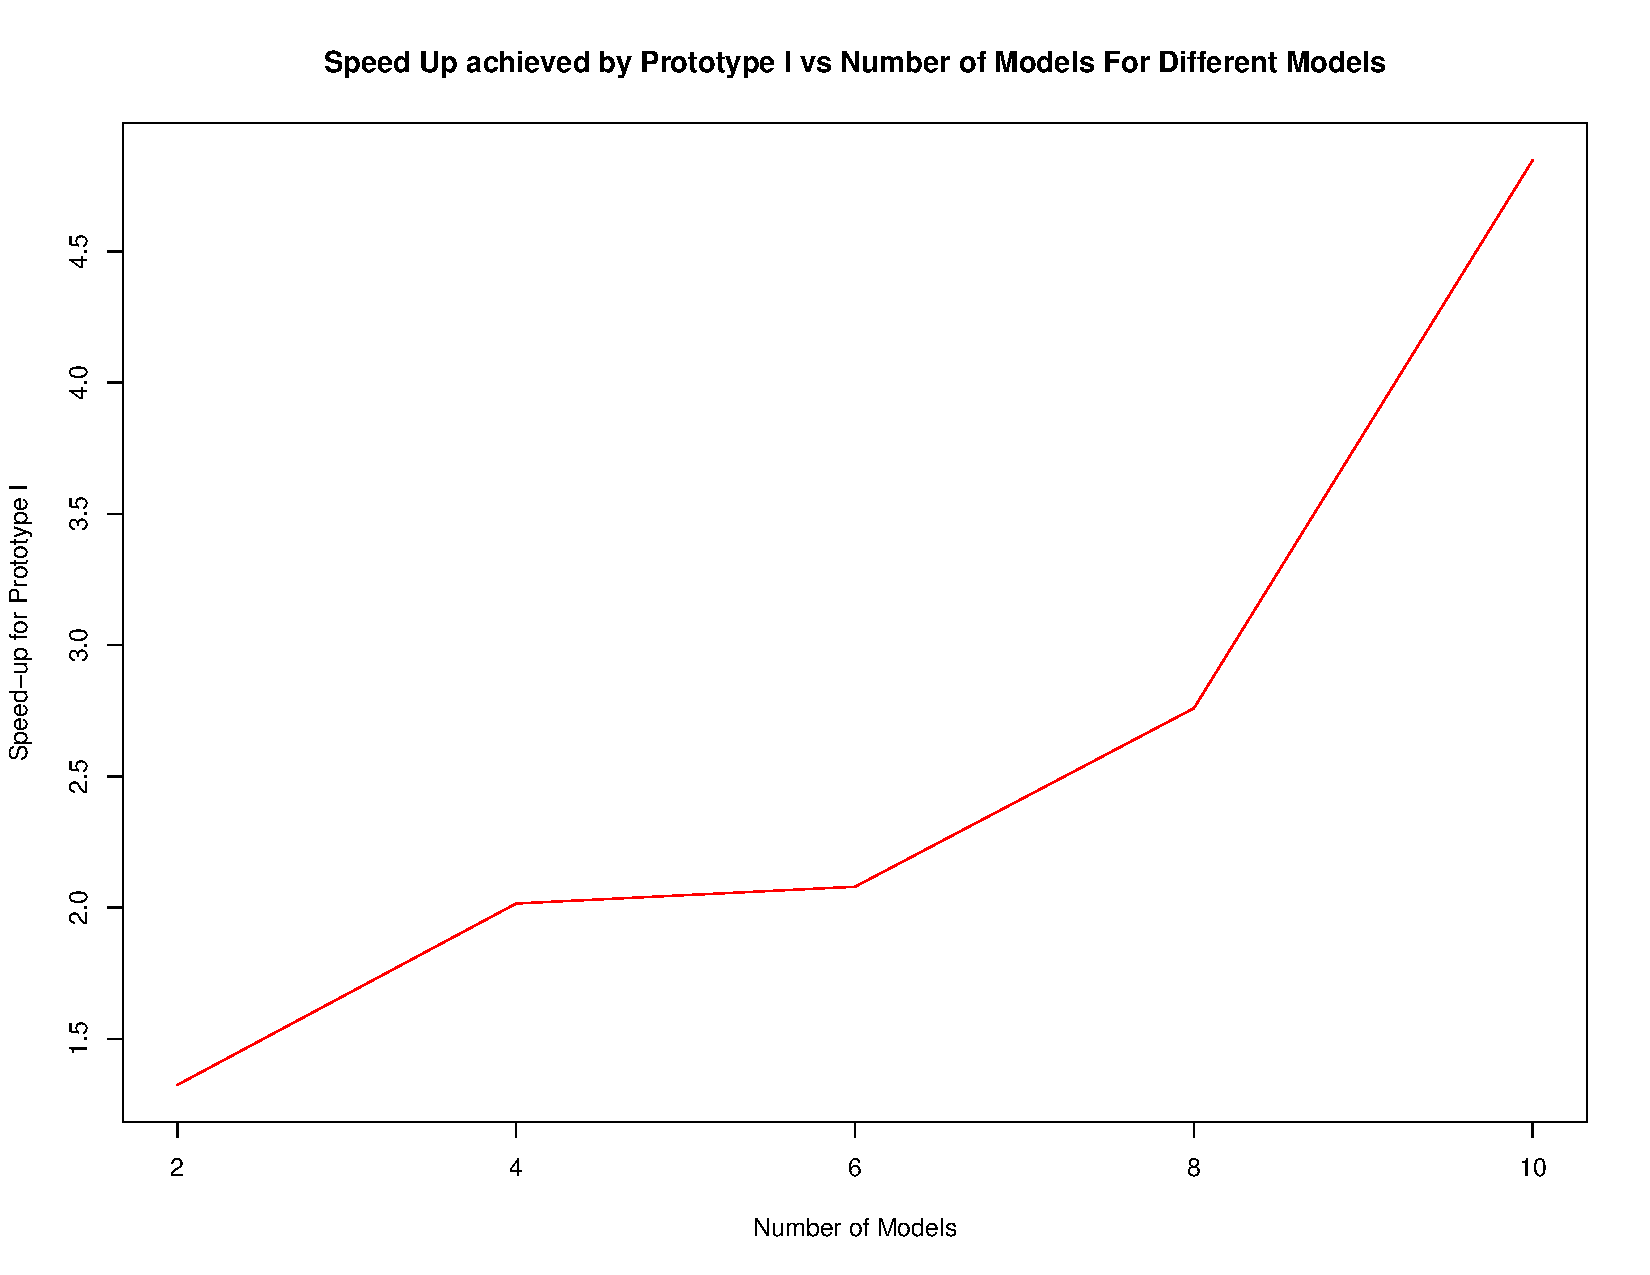
\includegraphics[scale=0.5]{SpeedUp-ProtoIDiffModelsVsNumModels.pdf}
\caption{Speed-up Vs Number of Models}
\label{fig:SpeedUp-ProtoIDiffModelsVsNumModels}
\end{subfigure}
\begin{subfigure}
\centering
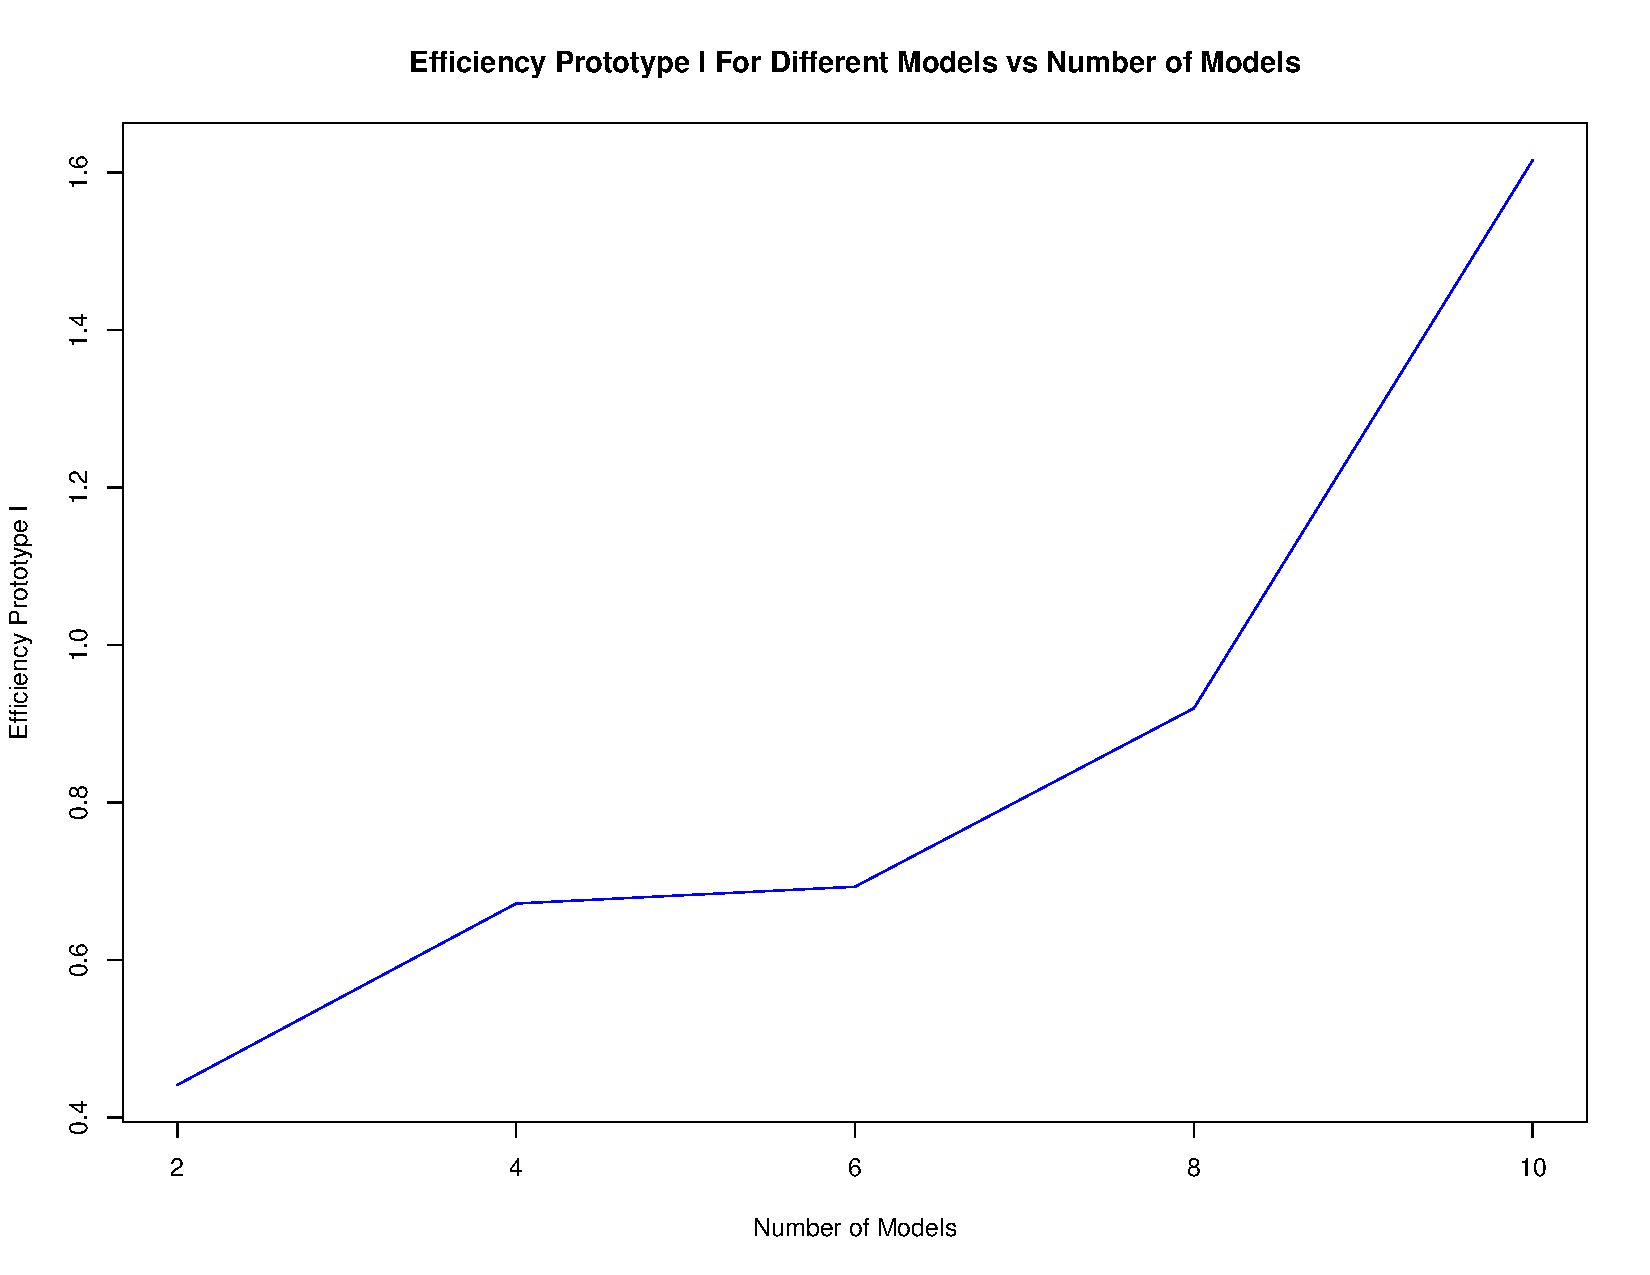
\includegraphics[scale=0.5]{Effi-ProtoIDiffModelsVsNumModels.pdf}
\caption{Efficiency Vs Number of Models}
\label{ProtoIDiffModelsVsNumModels}
\end{subfigure}
\end{figure}


\begin{equation}
\label{eq:NumVoxel}
\begin{aligned}
T_{NumVoxels} = (W\div voxDims.y) \times (L\div voxDims.x) \times (H \div voxDims.z)
\end{aligned}
\end{equation}


\subsubsection{Distributed Cuttlefish Prototype II vs Non-Distributed Cuttlefish}
To check the speed-up gained by using the Distributed Cuttlefish Prototype II, the application was run with different work-loads and comparison between the execution times for both Distributed Cuttlefish Prototype I and Non-Distributed Cuttlefish application was drawn.

\begin{enumerate}
\item{\textbf{Scenario}}- To test the computational speed-up gained by distributed cuttlefish prototype II in comparison to non-distributed cuttlefish for input consisting of same models.
\begin{itemize}
\item{\textbf{Test-Case and Test-Data Description}}- The test-case and the test-data used here is exactly same as the test-case and test-data of Scenario 1 of Prototype I testing.
\item{\textbf{Results}}- The amount of work done by the nodes remains same as described in Scenario 1 of Prototype I testing. The Table \ref{ProtoIISameModelsVsND} summarizes the execution time for the test case for prototype II.
\item{\textbf{Observation}}- The speed-up for the prototype II was calculated using the Equation \ref{eq:speed-up} and efficiency was calculated using the Equation \ref{eq:eff}. The Figure \ref{fig:ProtoIISpeedupVsNumModels} and Figure \ref{EfficiencyPrototIIvsNumModels} depict the trend seen for the speed-up and efficiency for prototype II. As the number of models increases the speed-up and efficiency increases for a given cluster size until a certain point (i.e. until the number of models reaches 8 models, at which there is peak performance seen) after which with increase in number of models the speed-up decreases and so does the efficiency.  
\end{itemize}

\item{\textbf{Scenario}}- To test the computational speed-up gained by distributed cuttlefish prototype II in comparison to non-distributed cuttlefish for input consisting of different models.
\begin{itemize}
\item{\textbf{Test-Case and Test-Data Description}}- The test-case and the test-data used here is exactly same as the test-case and test-data of Scenario 2 of Prototype I testing.
\item{\textbf{Results}}- The amount of work done by the nodes remains same as described in Scenario 2 of Prototype I testing. The Table \ref{ProtoIIDiffModelsVsND} summarizes the execution time for the test case for prototype II.
\item{\textbf{Observation}}-  The speed-up for the prototype II was calculated using the Equation \ref{eq:speed-up} and efficiency was calculated using the Equation \ref{eq:eff}. The Figure \ref{fig:SpeedUp-ProtoIIDiffModelsVsNumModels} and Figure \ref{Effi-ProtoIIDiffModelsVsNumModels} depict the trend seen for the speed-up and efficiency for prototype II for different models as input set. As the number of models increases the speed-up and efficiency increases.
\end{itemize}
\end{enumerate}


\begin{table}[]
\centering
\caption{Speed-Up \& Efficiency: Distributed Cuttlefish Prototype II vs Non-Distributed Cuttlefish for Same Models}
\label{ProtoIISameModelsVsND}
\begin{tabular}{|c|l|l|l|c|}
\hline
\textbf{\begin{tabular}[c]{@{}c@{}}Number of \\ Head -8 cm\\ (Resolution:\\ 300 X 150 X 470)\end{tabular}} & \multicolumn{1}{c|}{\textbf{\begin{tabular}[c]{@{}c@{}}Total Execution Time \\ (in secs)\\  for Distributed \\ Cuttlefish Prototype II\\ (Cluster Size- 3)\end{tabular}}} & \multicolumn{1}{c|}{\textbf{\begin{tabular}[c]{@{}c@{}}Total Execution Time\\ (in secs) \\ for Non-Distributed\\ Cuttlefish\end{tabular}}} & \multicolumn{1}{c|}{\textbf{Speed-Up}} & \textbf{Efficiency} \\ \hline
2                                                                                                          & 102.5524                                                                                                                                                                  & 357.355                                                                                                                                    & 3.484608844                            & 1.161536281         \\ \hline
4                                                                                                          & 245.0836                                                                                                                                                                  & 920.566                                                                                                                                    & 3.756130561                            & 1.25204352          \\ \hline
6                                                                                                          & 440.416                                                                                                                                                                   & 1651.177                                                                                                                                   & 3.749130368                            & 1.249710123         \\ \hline
8                                                                                                          & 708.706                                                                                                                                                                   & 4071.56                                                                                                                                    & 5.745062127                            & 1.915020709         \\ \hline
10                                                                                                         & 1014.9828                                                                                                                                                                 & 4790.198                                                                                                                                   & 4.719486872                            & 1.573162291         \\ \hline
\end{tabular}
\end{table}

\begin{table}[]
\centering
\caption{Speed-Up \& Efficiency: Distributed Cuttlefish Prototype II vs Non-Distributed Cuttlefish for Different Models}
\label{ProtoIIDiffModelsVsND}
\begin{tabular}{|c|c|c|c|c|}
\hline
\textbf{\begin{tabular}[c]{@{}c@{}}Number of \\ Head \& Dame,\\ Models -8 cm\\ (Resolution:\\ 300 X 150 X 470)\end{tabular}} & \textbf{\begin{tabular}[c]{@{}c@{}}Total Execution Time \\  (in secs) for \\ Distributed \\ Cuttlefish Prototype II\\ (Cluster Size- 3)\end{tabular}} & \textbf{\begin{tabular}[c]{@{}c@{}}Total Execution Time\\ (in secs) for \\ Non-Distributed\\ Cuttlefish\end{tabular}} & \textbf{Speed-up} & \textbf{Efficiency-ProtoII} \\ \hline
2                                                                                                                            & 94.52152                                                                                                                                              & 243.94                                                                                                                & 2.580787952       & 0.860262651                 \\ \hline
4                                                                                                                            & 181.9578                                                                                                                                              & 635.524                                                                                                               & 3.492699956       & 1.164233319                 \\ \hline
6                                                                                                                            & 357.616                                                                                                                                               & 1171.32                                                                                                               & 3.275356807       & 1.091785602                 \\ \hline
8                                                                                                                            & 492.6532                                                                                                                                              & 1890.706                                                                                                              & 3.837803144       & 1.279267715                 \\ \hline
10                                                                                                                           & 792.6886                                                                                                                                              & 4793.47                                                                                                               & 6.047103491       & 2.015701164                 \\ \hline
\end{tabular}
\end{table}

\begin{figure}
\centering
\captionsetup[subfigure]{labelformat=empty}
\begin{subfigure}
\centering
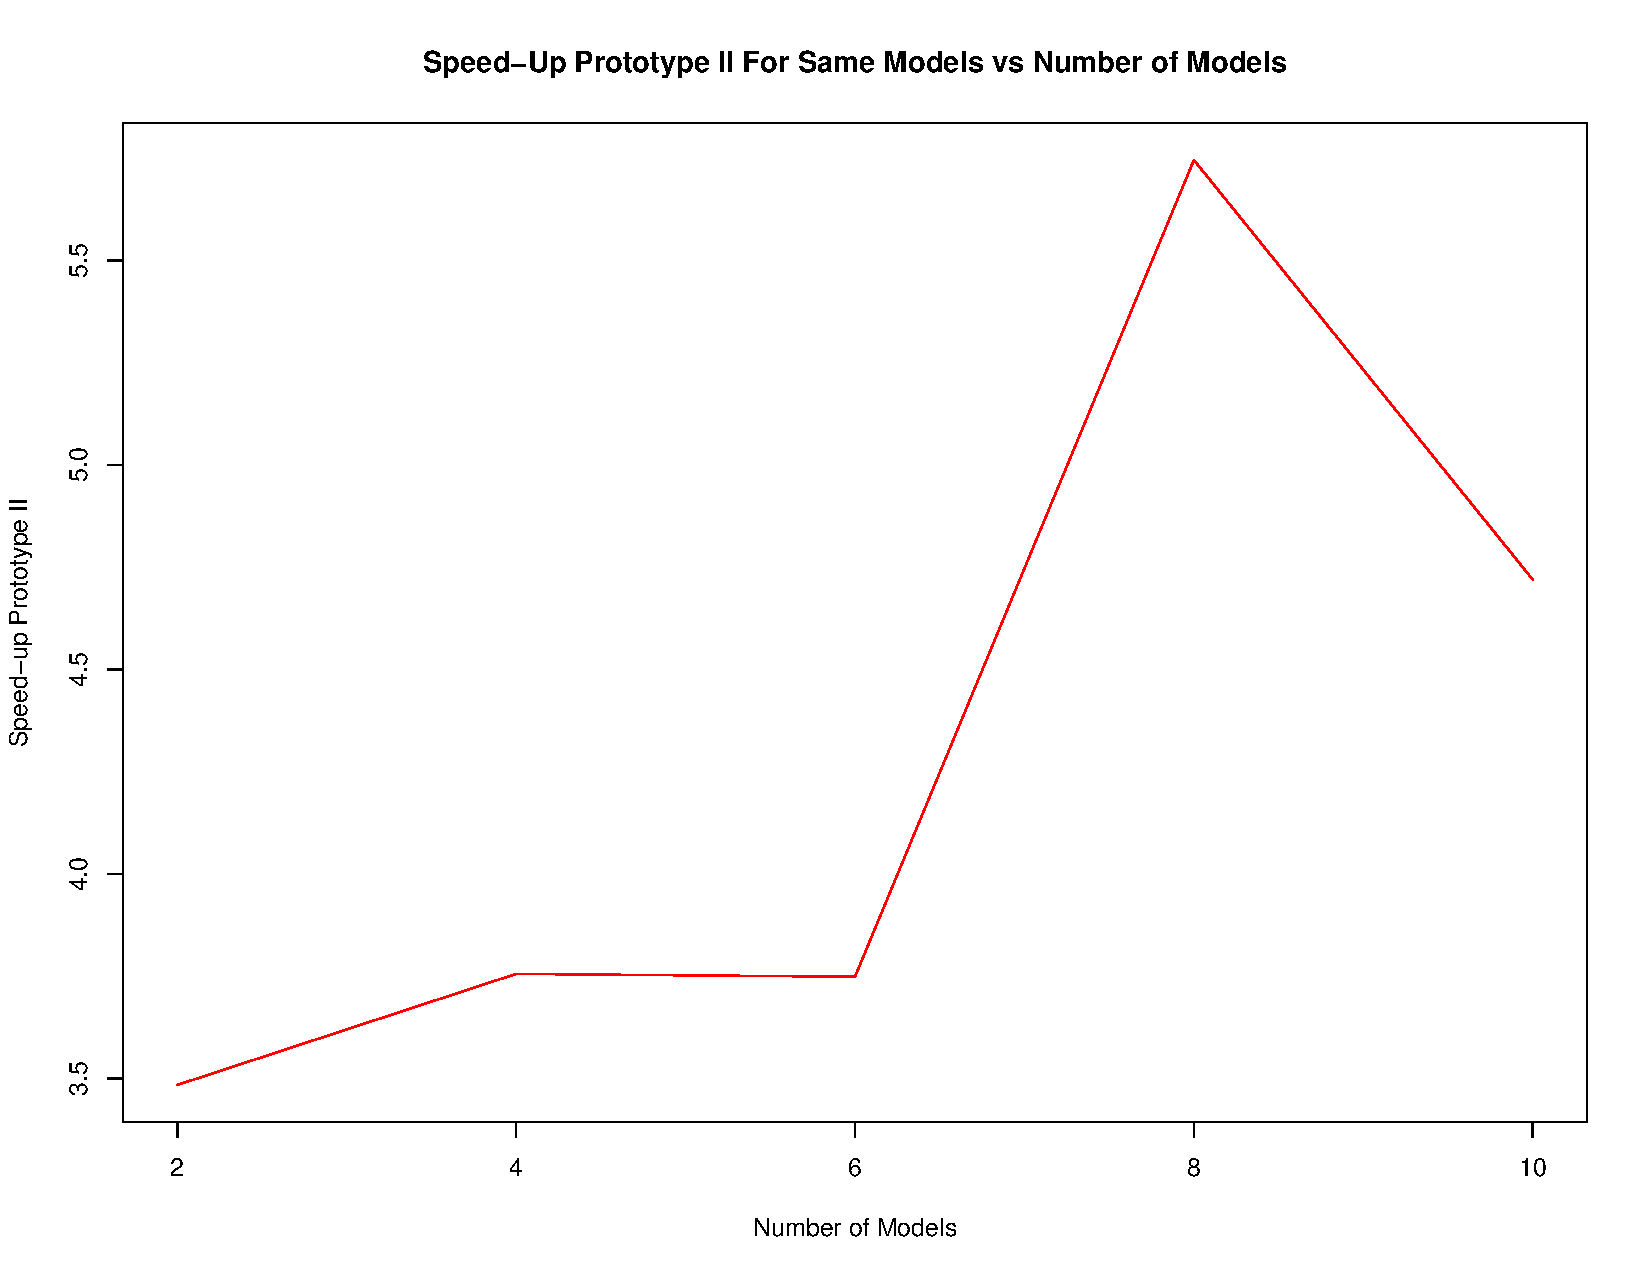
\includegraphics[scale=0.5]{ProtoIISpeedupVsNumModels.pdf}
\caption{Speed-up Vs Number of Models}
\label{fig:ProtoIISpeedupVsNumModels}
\end{subfigure}
\begin{subfigure}
\centering
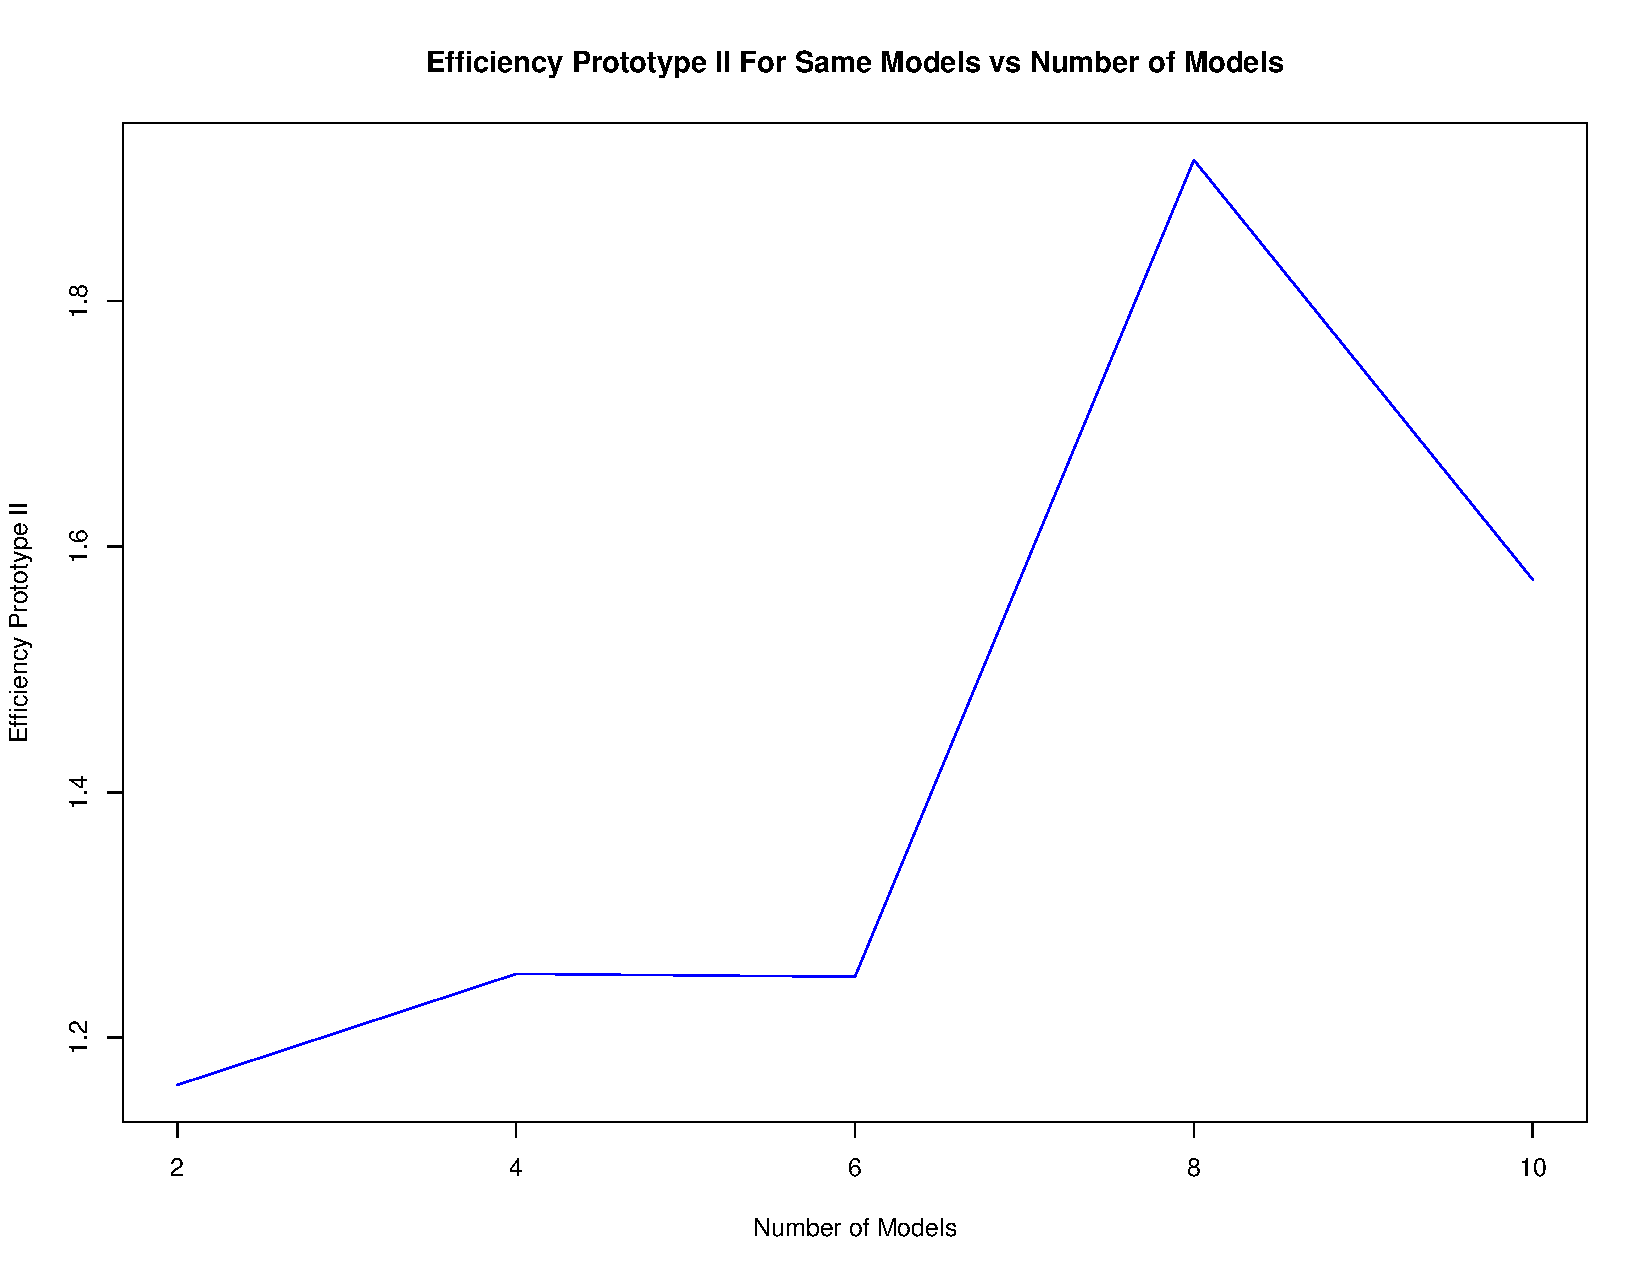
\includegraphics[scale=0.5]{EfficiencyPrototIIvsNumModels.pdf}
\caption{Efficiency Vs Number of Models}
\label{EfficiencyPrototIIvsNumModels}
\end{subfigure}
\end{figure}


\begin{figure}
\centering
\captionsetup[subfigure]{labelformat=empty}
\begin{subfigure}
\centering
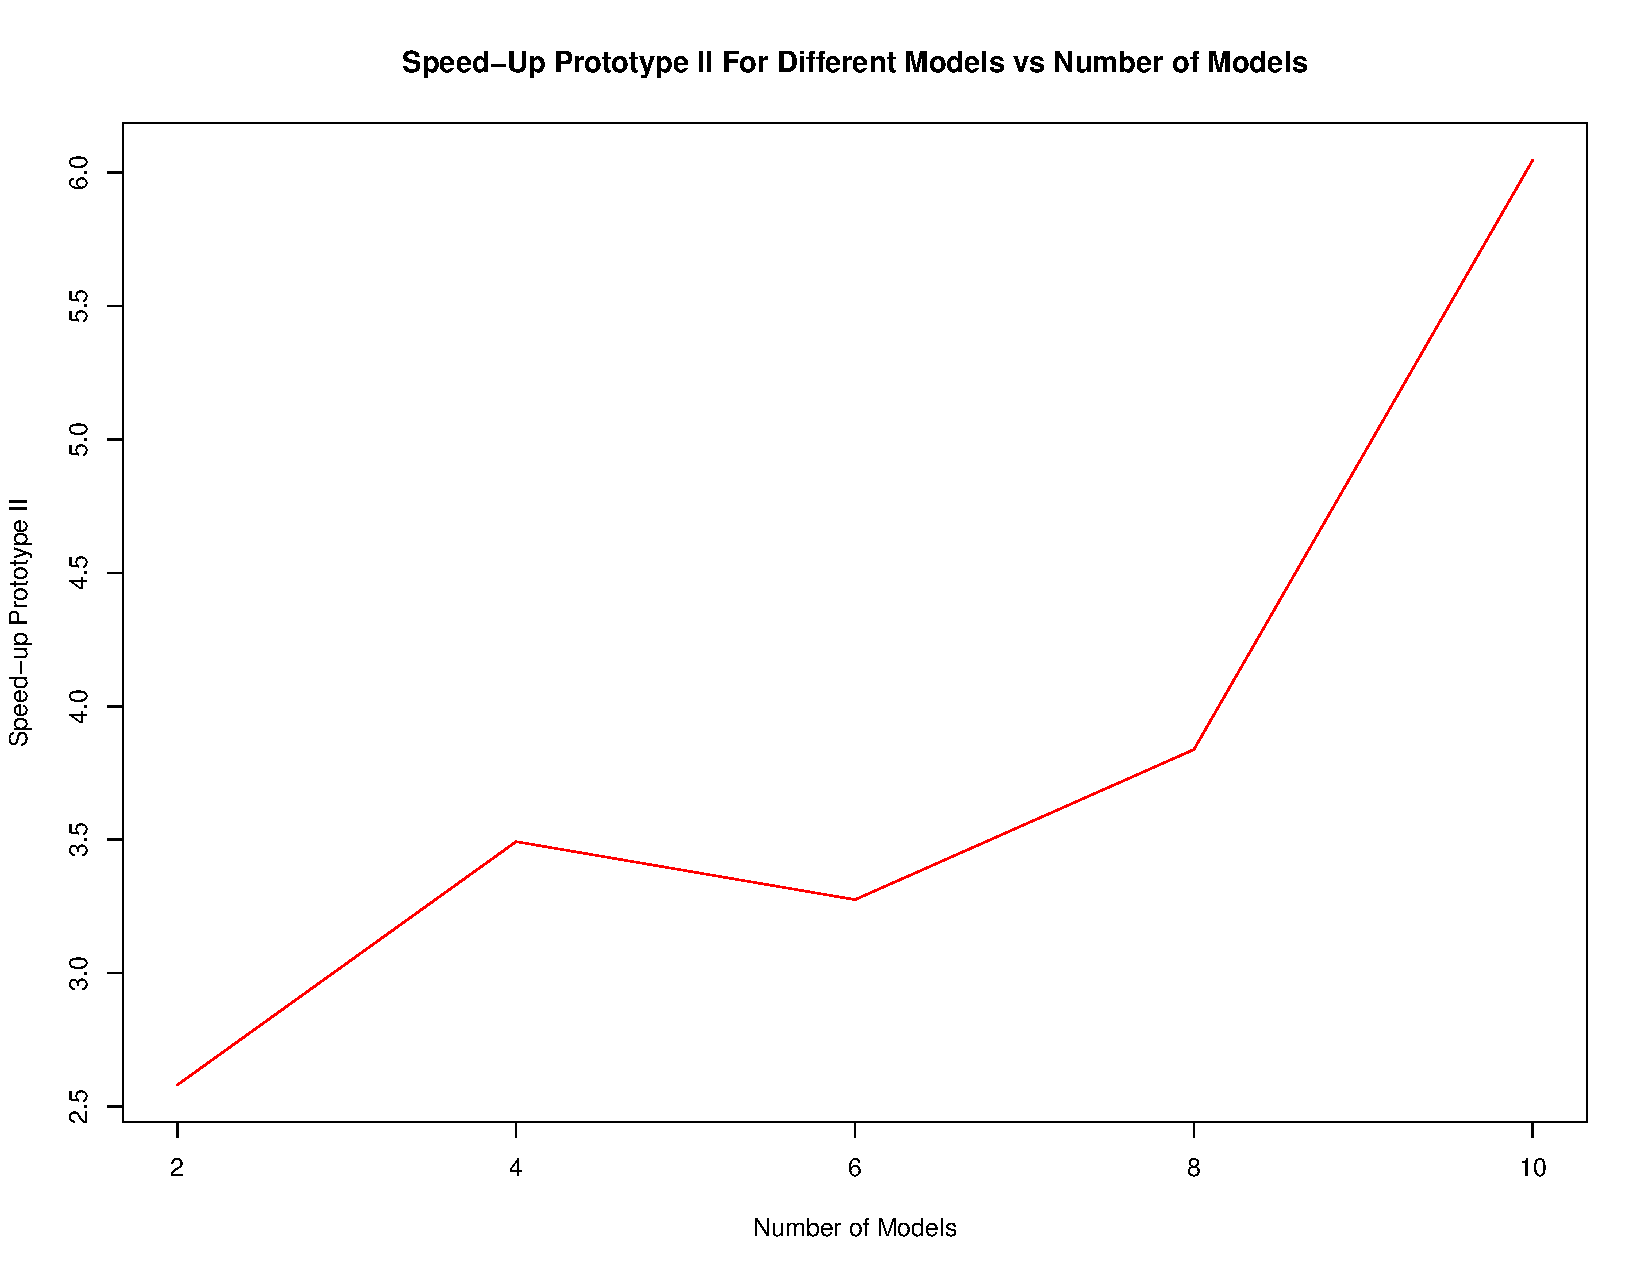
\includegraphics[scale=0.5]{SpeedUp-ProtoIIDiffModelsVsNumModels.pdf}
\caption{Speed-up Vs Number of Models}
\label{fig:SpeedUp-ProtoIIDiffModelsVsNumModels}
\end{subfigure}
\begin{subfigure}
\centering
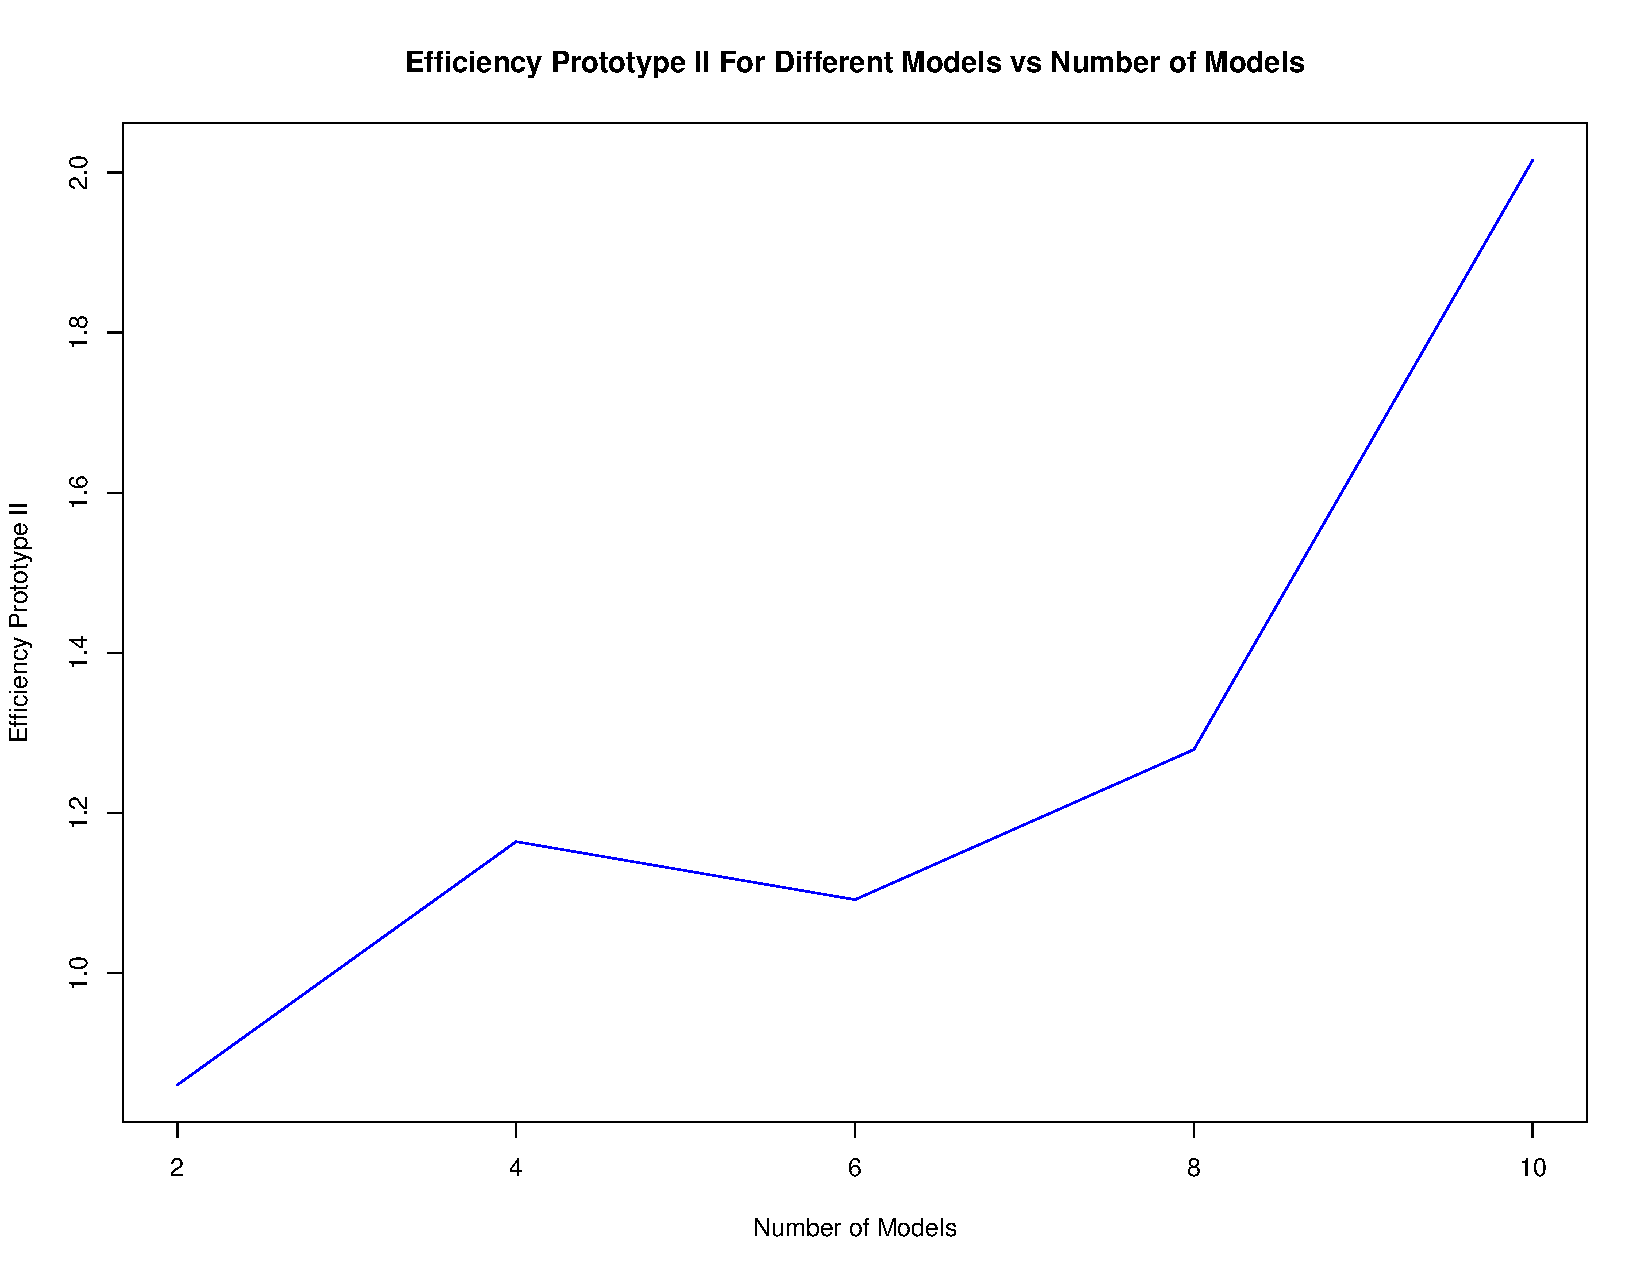
\includegraphics[scale=0.5]{Effi-ProtoIIDiffModelsVsNumModels.pdf}
\caption{Efficiency Vs Number of Models}
\label{Effi-ProtoIIDiffModelsVsNumModels}
\end{subfigure}
\end{figure}


\subsection{Comparison of Distributed Cuttlefish prototypes} \label{ProtoComp}


  